%!TEX root = ./main.tex
%!TEX encoding = UTF-8 Unicode
\chapter{Modélisation du jeu d'instruction}
\section{Modélisation sous 3 vues}
\label{sec:modelisationArborescente}
\subsection{Une modélisation arborescente}
\harmless\ utilise 3 vues pour décrire le jeu d'instruction d'un processeur:
\begin{itemize}
\item la vue binaire (\emph{format}) est utilisée pour décrire le format binaire des instructions, afin de permettre l'étape de décodage des instructions;
\item la vue comportementale (\emph{behavior}) permet de décrire le comportement des instructions, afin de simuler le comportement des instructions;
\item la vue syntaxique (\emph{syntax}) permet de décrire le mnémonique de l'instruction, afin de générer le désassembleur.
\end{itemize}

Chaque vue est un ensemble d'arbre, où chaque n\oe ud décrit une partie de \emph{format}, \emph{behavior} ou \emph{syntax}. La description d'un n\oe ud se fait de la manière suivante:
\begin{verbatim}
<kind> <name> <kind_options>
  <kind_body>
end <kind>
\end{verbatim}
où \texttt{<kind>} peut être \texttt{format}, \texttt{behavior} ou \texttt{syntax}. Par défaut, un n\oe ud agrège les sous n\oe uds qui sont définis dans sont corps. Toutefois, la construction autour du mot clé \texttt{select} permet, dans chaque vue, de choisir un sous n\oe ud parmi plusieurs.

Cette approche arborescente a pour objectif de factoriser au maximum les éléments similaires (au niveau de la syntaxe, du comportement ou du format binaire).

En utilisant ce modèle, dans chaque vue, une instruction est représentée par une branche dans un arbre. Les instruction qui partagent certains caractéristiques dans une vue partagent les même n\oe uds de la racine de l'arbre, tandis que les parties spécifiques se retrouvent dans les feuilles.

\subsection{Signature d'une instruction}
\label{sec:signature}
Un n\oe ud peut avoir une ou plusieurs étiquettes. Une étiquette est représentée dans \harmless\ par le caractère \texttt{\#} suivi d'une chaîne alphanumérique. 

\emph{L'ensemble} des étiquettes le long d'une branche d'un arbre est l'identifiant unique d'une instruction et est appelé la \emph{signature de l'instruction}. La signature est un ensemble d'étiquette, ce qui implique qu'il n'y a pas de notion d'ordre, et qu'il n'y a pas de comptage du nombre d'occurrence de chaque étiquette.

Dans certains cas, il est utile de pouvoir \emph{marquer} des étiquettes car un même n\oe ud peut être utilisé dans des contextes différents, par exemple lors de la lecture de 2 registres source d'une instruction. Dans ce cas, on utilise une \emph{post-étiquette}. Une post-étiquette est représentée par le caractère \texttt{@} suivi d'une chaine de caractère. Il à pour conséquence de modifier toutes les étiquettes du sous arbre en rajoutant comme suffixe la post-étiquette (sans le caractère \texttt{@}).

C'est ce mécanisme qui est utilisé pour faire le lien d'une instruction selon différentes vues.

\subsection{Un exemple}
\label{exempleSignature}
Les exemples seront expliqués plus en détails dans les chapitres traitants des différentes vues. L'objectif ici est de montrer comment se définit la structure arborescente.

Considérons par exemple le code (simplifié) suivant:
\begin{lstlisting}
behavior readGPR #read8
  ...
end behavior

behavior writeGPR #write8
  ...
end behavior

-- instruction that operate on 2 source registers
behavior twoRegsOp
  -- read the 2 source registers
  readGPR@src1
  readGPR@src2
  select
    case #ADC  ...
    case #ADD  ...
    case #SUB  ...
  end select
  writeGPR
end behavior

\end{lstlisting}
Cet exemple décrit 3 n\oe uds (non terminaux) de type \texttt{behavior}: \texttt{readGPR}, \texttt{writeGPR}, et \texttt{twoRegsOp}. Le n\oe ud \texttt{twoRegsOp} est la racine de l'arbre, car il n'est appelé dans aucun autre n\oe ud. 

\begin{figure}		%% Small Example
  \begin{center}
    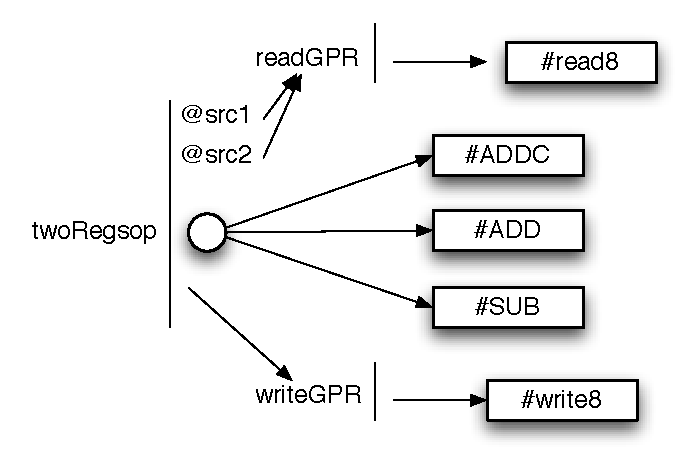
\includegraphics[width=0.8 \linewidth]{../common/images/instBase.pdf}
    \caption{Représentation arborescente de l'arbre décrit dans l'exemple simple.}
    \label{fig:instBase}
  \end{center}
\end{figure}

Il est représenté graphiquement dans le schéma \ref{fig:instBase}. Chaque n\oe ud est représenté par son nom, ainsi que par une barre verticale. À droite de la barre verticale, les différents "élements" (structure de sélection, appel d'un autre n\oe ud avec ou sans \emph{post-étiquette}) sont indiqués \emph{séquentiellement}. Le cercle permet de représenter le structure de sélection (\texttt{select}). Les \emph{étiquettes} sont représentées dans des rectangles, et les \emph{post-étiquettes} sont représentées dans le n\oe ud appelant.

L'intérêt d'utiliser ici une \emph{post-étiquettes} tient dans le fait que le n\oe ud \texttt{readGPR} est appelé dans 2 contextes différents: un pour chaque registre source. Comme la \emph{post-étiquettes} est ajoutée à chaque \emph{étiquette} du sous-arbre, il y a bien une différenciation: \texttt{\#read8src1} et \texttt{\#read8src2}.

Ainsi dans cet exemple, l'instruction ADD a comme ensemble d'étiquettes:  \texttt{\#read8src1}, \texttt{\#read8src2}, \texttt{\#ADD} et \texttt{\#write8}. De même, l'instruction SUB a comme ensemble d'étiquette:  \texttt{\#read8src1}, \texttt{\#read8src2}, \texttt{\#SUB} et \texttt{\#write8}. Cette ensemble d'étiquette constitue la signature de l'instruction.

Au niveau fonctionnement interne, chaque instruction est associée à une classe $C++$, le nom de la classe sera ici \texttt{cpu\_ADD\_read8src1\_read8src2\_write8}. Pour définir le nom interne de l'instruction, on concatène le nom du modèle (ici \texttt{cpu}) avec les différentes étiquettes séparées par le caractère '\texttt{\_}', dans l'ordre alphabétique.

%\subsection{Intérêt de la structure selon 3 vues}
%TODO 
